\documentclass[../main.tex]{subfiles}

\begin{document}
\section{Results}
The results' section presents the findings from the analysis of
the accelerometer data collected during the simulated intrusion attempts
on the MediColbox.
The accelerometer data provides insights into the physical movements
and vibrations experienced by the MediColbox during these intrusion scenarios.

\subsection{Analysis of Accelerometer Data}

The accelerometer data captured the acceleration patterns resulting from different simulated intrusion attempts, including striking, dropping, sawing, and shaking the MediColbox.
The data analysis focused specifically on the accelerometer readings to evaluate the sensitivity and effectiveness of the IMU in detecting unauthorized access.

\clearpage

\subsubsection{Striking the MediColbox}

Figure \ref{fig:accelerometer_striking} presents the
accelerometer data recorded when the MediColbox was
struck with a fist.
The accelerometer readings showed a sharp increase in
acceleration followed by a swift, but gradual decrease as
the impact dissipated.
The peak acceleration value reached during the
strike was measured at
$X = 5 [m/s^2]$, $Y = -31 [m/s^2]$, $Z = -55 [m/s^2]$
and occurred at $t = 0.8[s]$.
The analysis of the data indicates that the
IMU successfully detected and recorded the impact caused by the
striking event.

\begin{figure}[htbp]
    \centering
    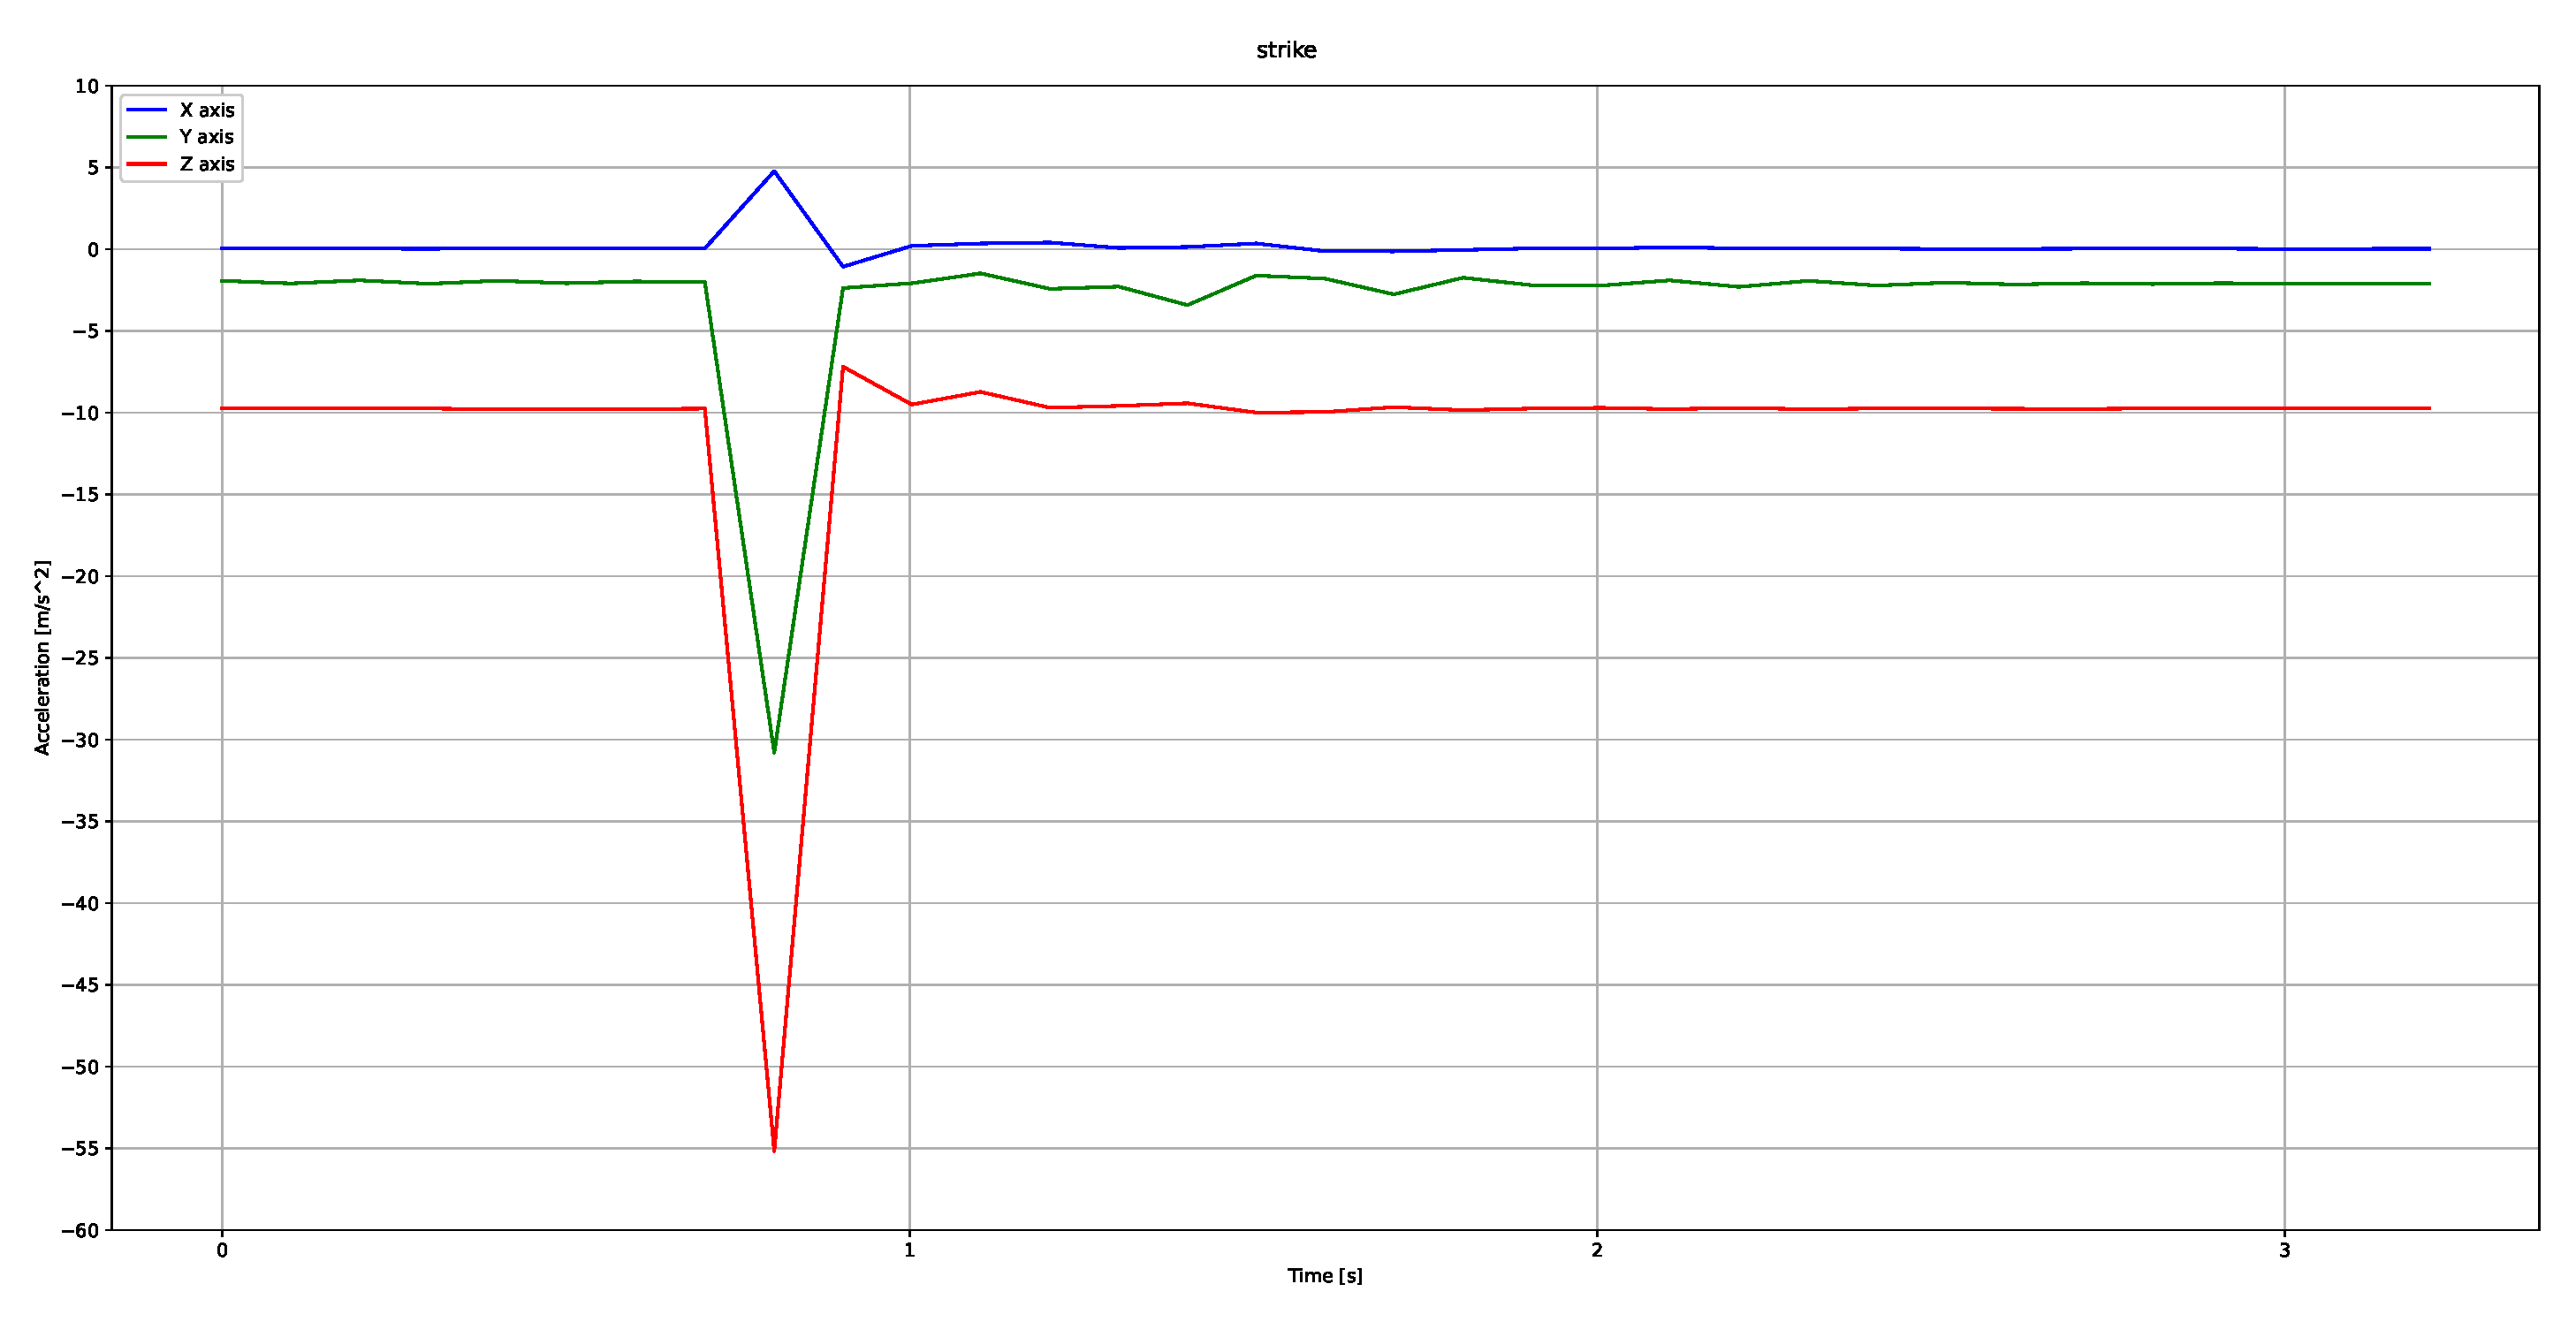
\includegraphics[width=0.8\textwidth]{resources/figures/Acceleration_strike.eps}
    \caption{Accelerometer data during the striking event}
    \label{fig:accelerometer_striking}
\end{figure}

Looking at the data we can clearly see the peak acceleration and how it
stands out from the rest of the data visualized. However,
how do we set criteria so that we can automatically claim
an acceleration like this is an attempt of intrusion and not just a random event? A way we, during the data gathering, could reason for, was to find the force needed to break the box and estimate from the weight of the box how much acceleration would be close to breaking the box open. In this case the data gathering "Protoype" is $0.645 [kg]$. With the measured acceleration in $X$, $Y$ and $Z$ direction results in a combined acceleration of $|\overrightarrow{a}| = \sqrt{5^2+(-32)^2+(-55)^2} [m/s^2] \approx 63.332 [m/s^2]$. If a box is designed to handle an impact large enough to momentary expose it to $63.332 [m/s^2]$ multiplied by a given safety factor, then it would be viable to account for sensor error margins and say that any acceleration above $60 [m/s^2]$ should immediately trigger an alarm.

Another method could be to assume that if somebody wanted to break the box, they would either break the box in one strike, or try to hit the box repeatedly with strikes that individually might not break the box but that combined might manage to break the bx due to material fatigue. If we divide the strike force that would immediately trigger an alarm (in this case $60 [m/s^2]$), by the estimated resistance to fatigue in a scale from 0 to 1 and raise it to the number of strikes you assume you would need to break the box using the assumed amount of needed repeated strikes. An example of this could be to do the calculation:

$$a_{trigger} * {\rho_{fatigue}}^{n_{strikes}} \rightarrow 60 [m/s^2] * 0.9^5 \approx 35.43 [m/s^2] $$

In this example then $5$ repeated strikes of approximately $35.43 [m/s^2]$ will also trigger an alarm.

If we continue to analyze the data, we can try using frequency analysis on the striking event hoping to find information not revealed by just graphing the data. One way to find the frequency values of the data to analyze is using Fourier analysis. Herein this figure \ref{fig:fourier_accelerometer_striking}.
The Fourier analysis reveals to us the frequency components present in the accelerometer readings. This could
provide insights into the characteristics of the
impact and resulting vibrations.

\begin{figure}[htbp]
    \centering
    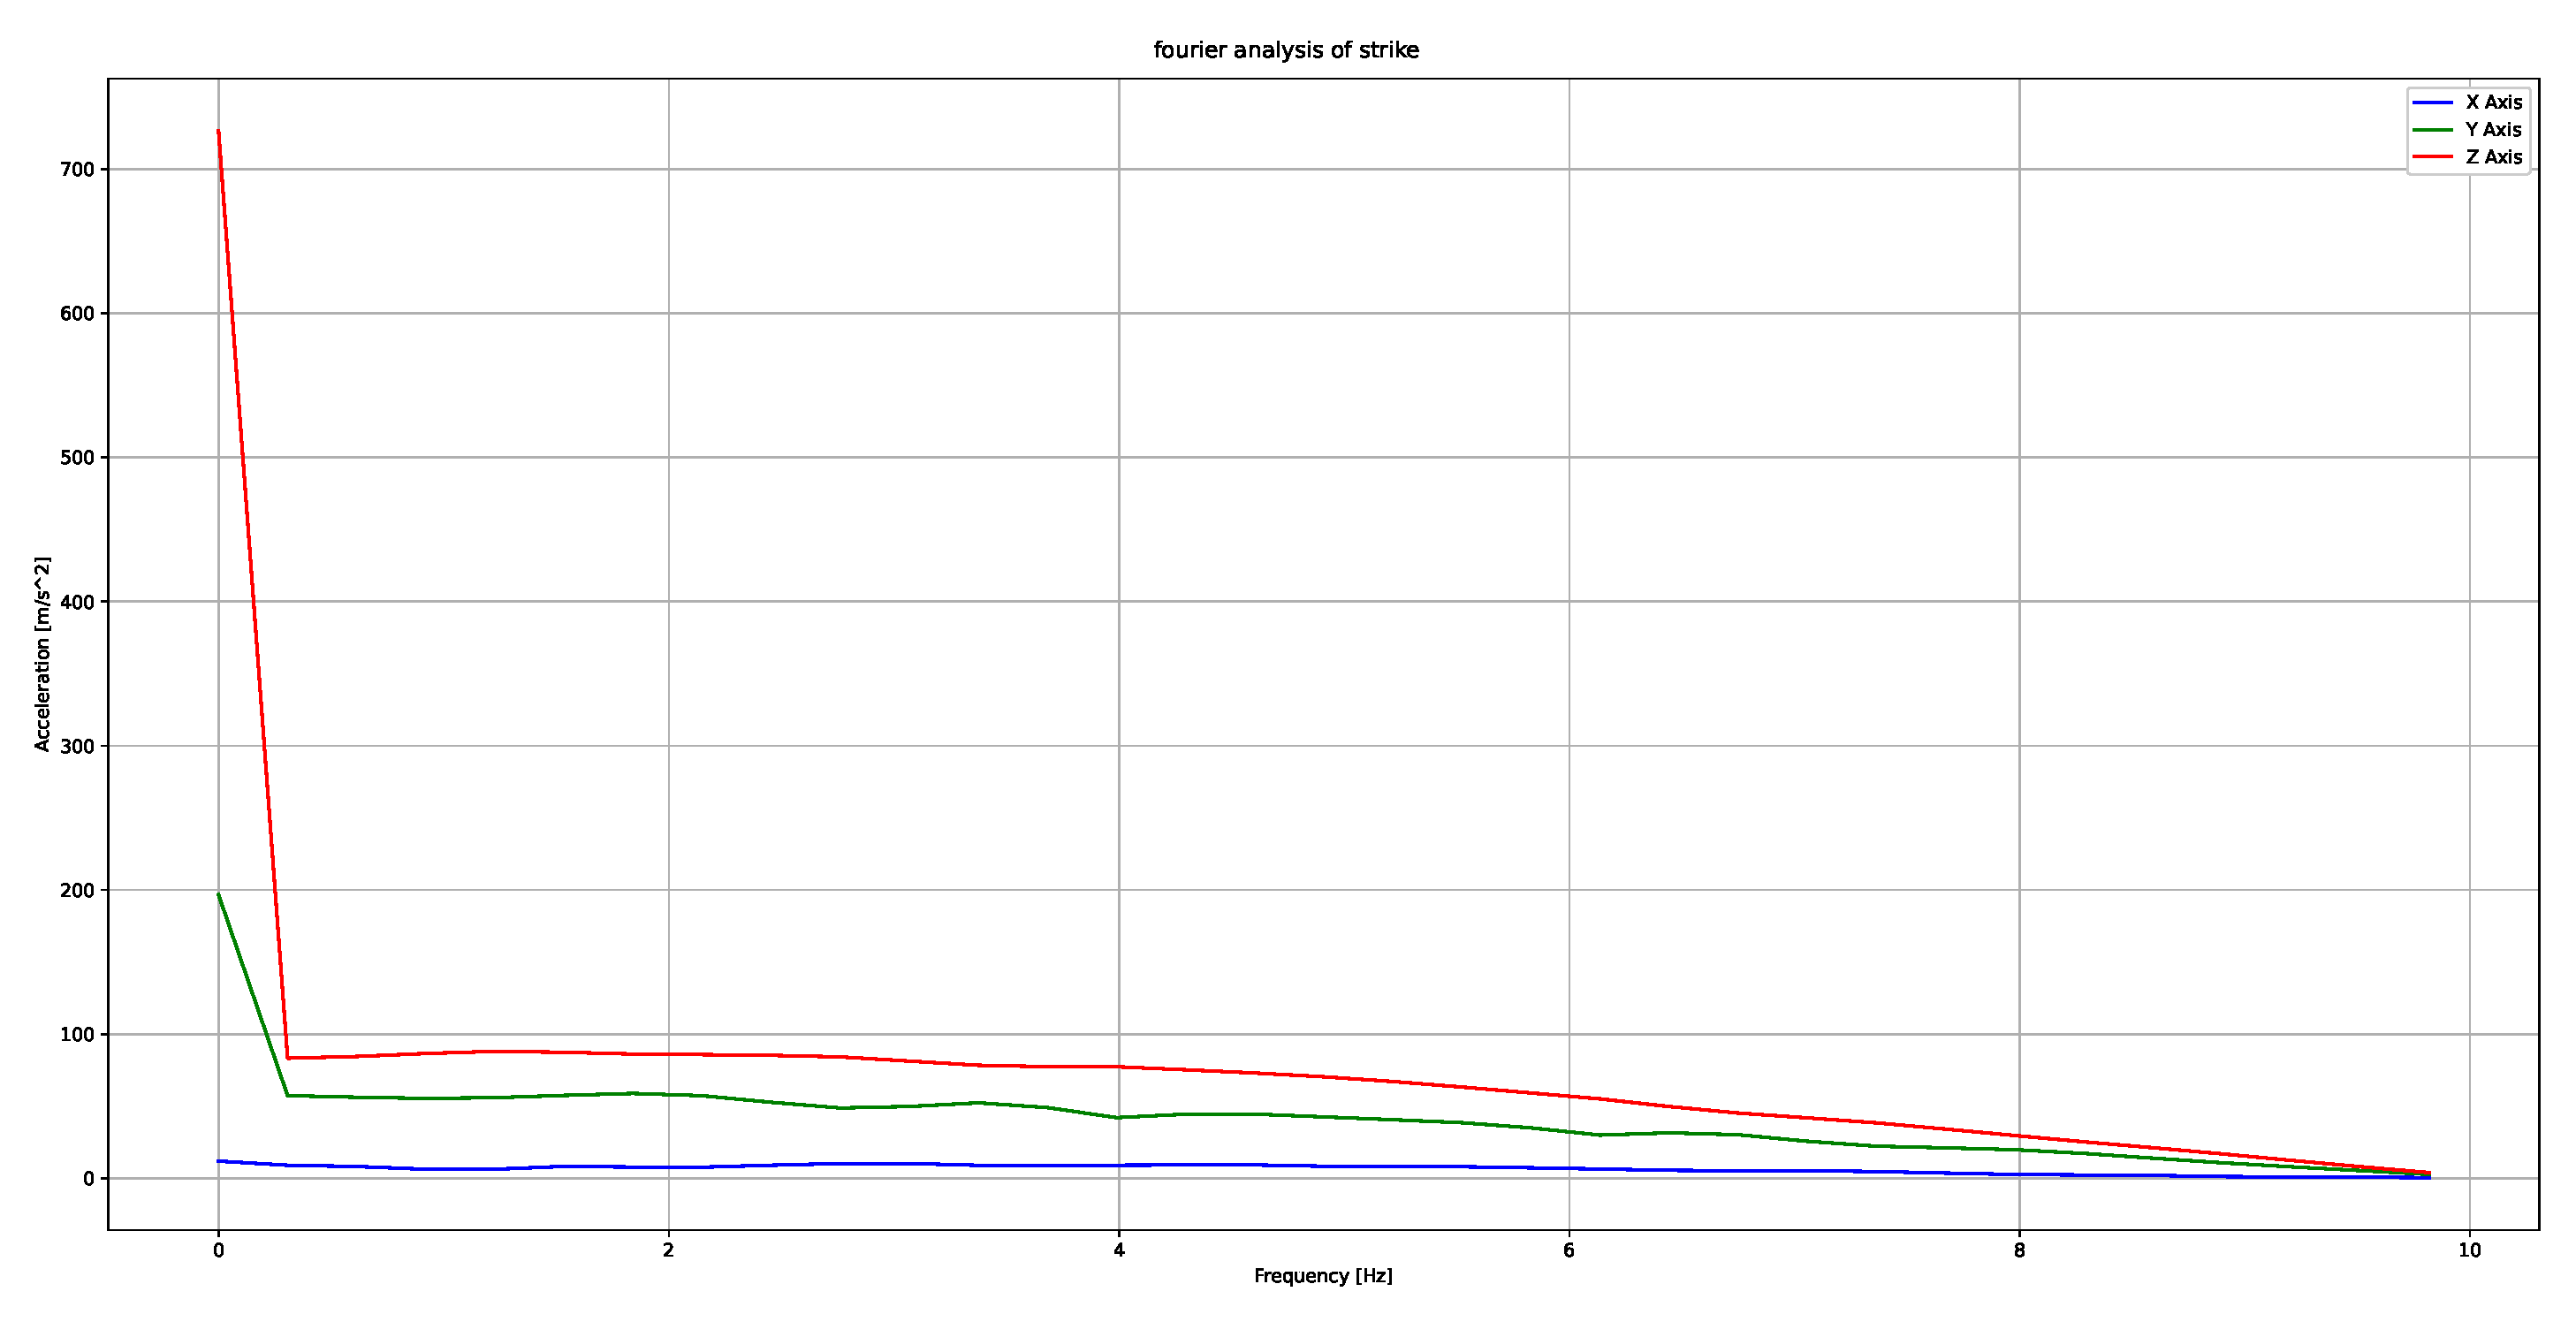
\includegraphics[width=0.8\textwidth]{resources/figures/Fourier_acceleration_strike.eps}
    \caption{Fourier analysis of accelerometer data during the striking event}
    \label{fig:fourier_accelerometer_striking}
\end{figure}

Looking at the Fourier transformed data no additional information could be extrapolated from the data, that wasn't already discussed from the untransformed data.

\clearpage
\subsubsection{Dropping the MediColbox}

The accelerometer data, collected when the MediColbox was slowly and carefully
pushed off of a table, is presented in
Figure \ref{fig:accelerometer_dropping}.
The maximum acceleration value recorded during the
drop was
$X = -7.7 [m/s^2]$, $Y = 35 [m/s^2]$, $Z = -50.7 [m/s^2]$,
which occurred at $t = 5.1[s]$.
The analysis confirms that the IMU effectively captured the
acceleration changes associated with the dropping event.

\begin{figure}[htbp]
    \centering
    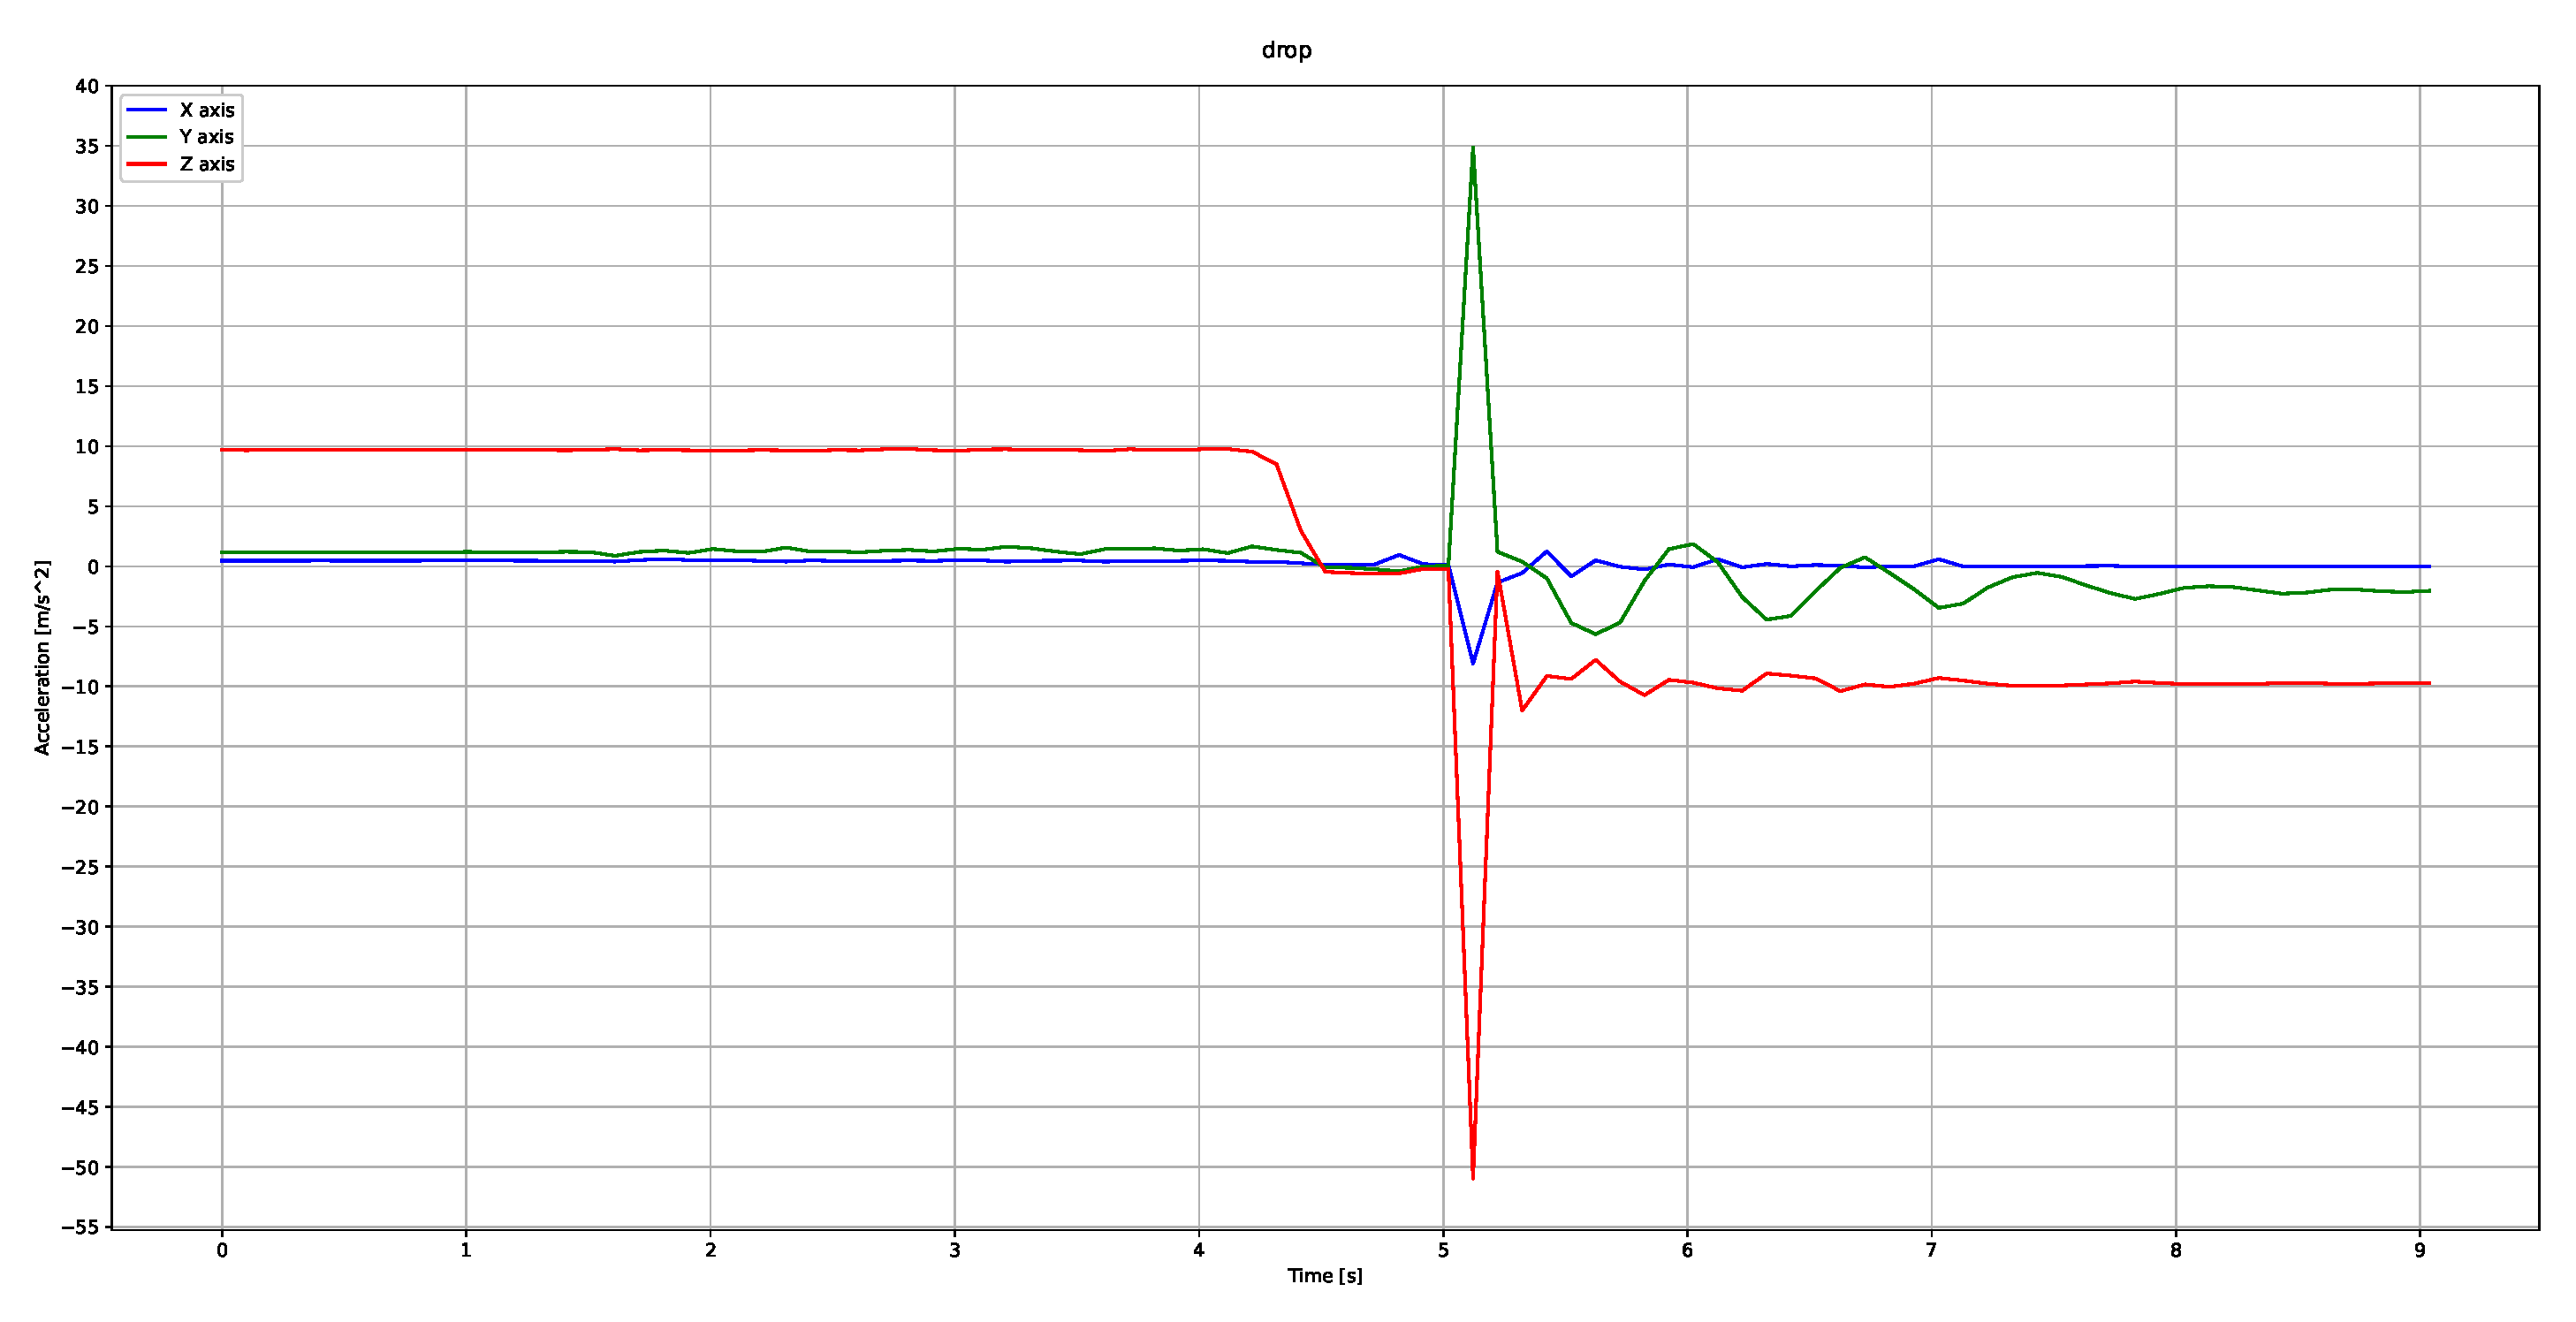
\includegraphics[width=0.8\textwidth]{resources/figures/Acceleration_drop.eps}
    \caption{Accelerometer data during the dropping event}
    \label{fig:accelerometer_dropping}
\end{figure}

Analyzing the data similarly to how we did at the striking event we find that in this case we have a total peak acceleration of $|\overrightarrow{a}| \approx 62 [m/s^2]$ this would already trigger the previously set trigger criteria of $60 [m/s^2]$, also, if we continue looking we see that approximately $t=5$ there appears to be no acceleration meassured, this is what is called a "free-fall" a reference frame of which no acceleration is observed to those in the free-falling frame of reference. \cite{Freefall_Encyclopædia_Britannica_2024}. However, looking at the gyroscope data from Figure \ref{fig:gyroscope_dropping} we can see that there is also a lot of rotational movement starting as early as $t=4$ this suggests that the Prototype is rolling of the edge of where it was dropped from.

\begin{figure}[htbp]
    \centering
    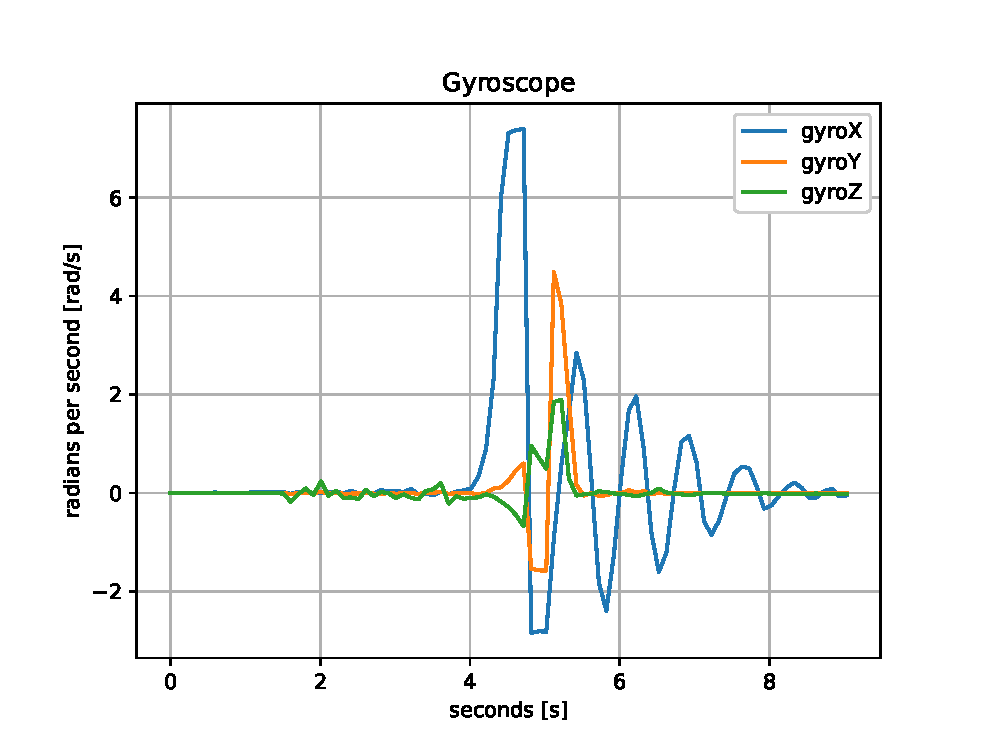
\includegraphics[width=0.8\textwidth]{resources/figures/Gyro_drop.eps}
    \caption{Gyroscope data during the dropping event}
    \label{fig:gyroscope_dropping}
\end{figure}

If we integrate the Gyroscope's angular velocity over time to make position we get an estimate of pose visualized in Figure \ref{fig:pose_dropping}.


\begin{figure}[htbp]
    \centering
    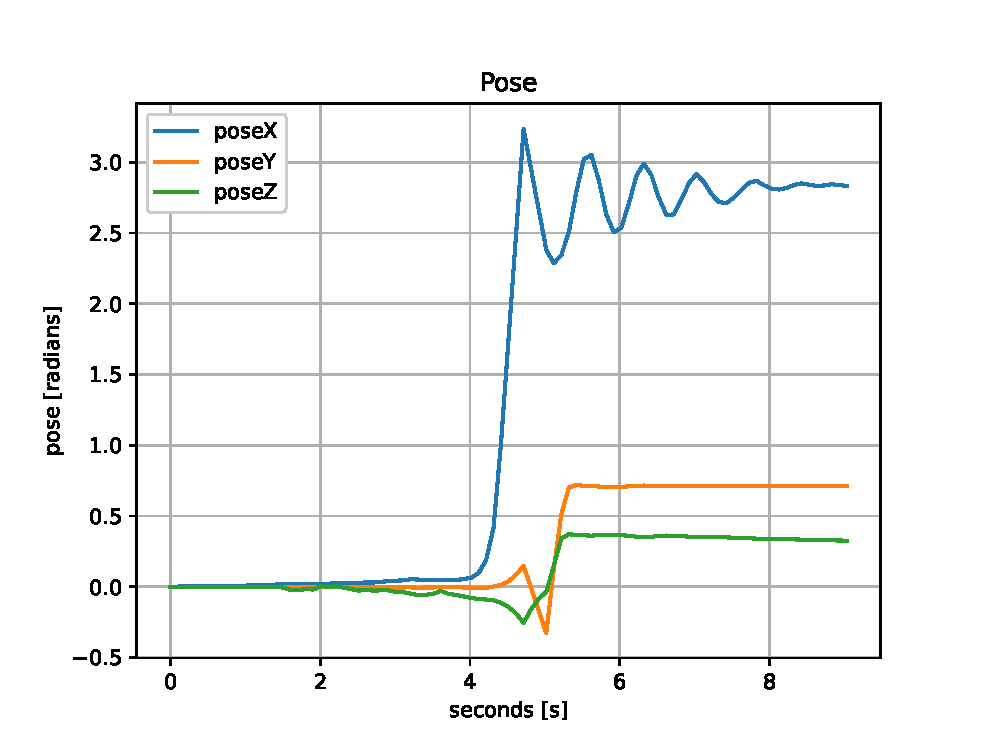
\includegraphics[width=0.8\textwidth]{resources/figures/Pose_drop.eps}
    \caption{Pose estimate during the dropping event}
    \label{fig:pose_dropping}
\end{figure}

In the pose data we notice that the estimated pose changes by approximately $3.1 [rad]$ (about $180$ degrees) in between time $t=4$ and $t=4.7$ this strongly suggest that the Protoype has roled half a round around the $X$-axis. This is supported in how the acceleration (Figure \ref{fig:accelerometer_dropping}) shows the $Z$-axis changes from being positive to being negative.
The pose changing in such drastic ways will be representative of how a box can be tipped over or turned around during an intrusion attempts when an intruder tries to figure out where to attack. Integrating position and velocity from acceleration and pose is also possible and combining the accumulated change in pose and the accumulated change in change of position might be valuable when the box wants to detect if somebody picks up the box and/or moves it to somewhere it shouldn't be. Using this we could theoretically set an area of where box is restricted to be within or outside.

A problem with this is that differentiating between intrusion attempts and just any random regular use is near impossible, and combined with how accumulating values also result in accumulated error. This makes any estimate less accurate over time


Movingon to the Fourier analysis of the accelerometer data during the
dropping event (Figure \ref{fig:fourier_accelerometer_dropping}.)
Here there is again little information to gain.

\begin{figure}[htbp]
    \centering
    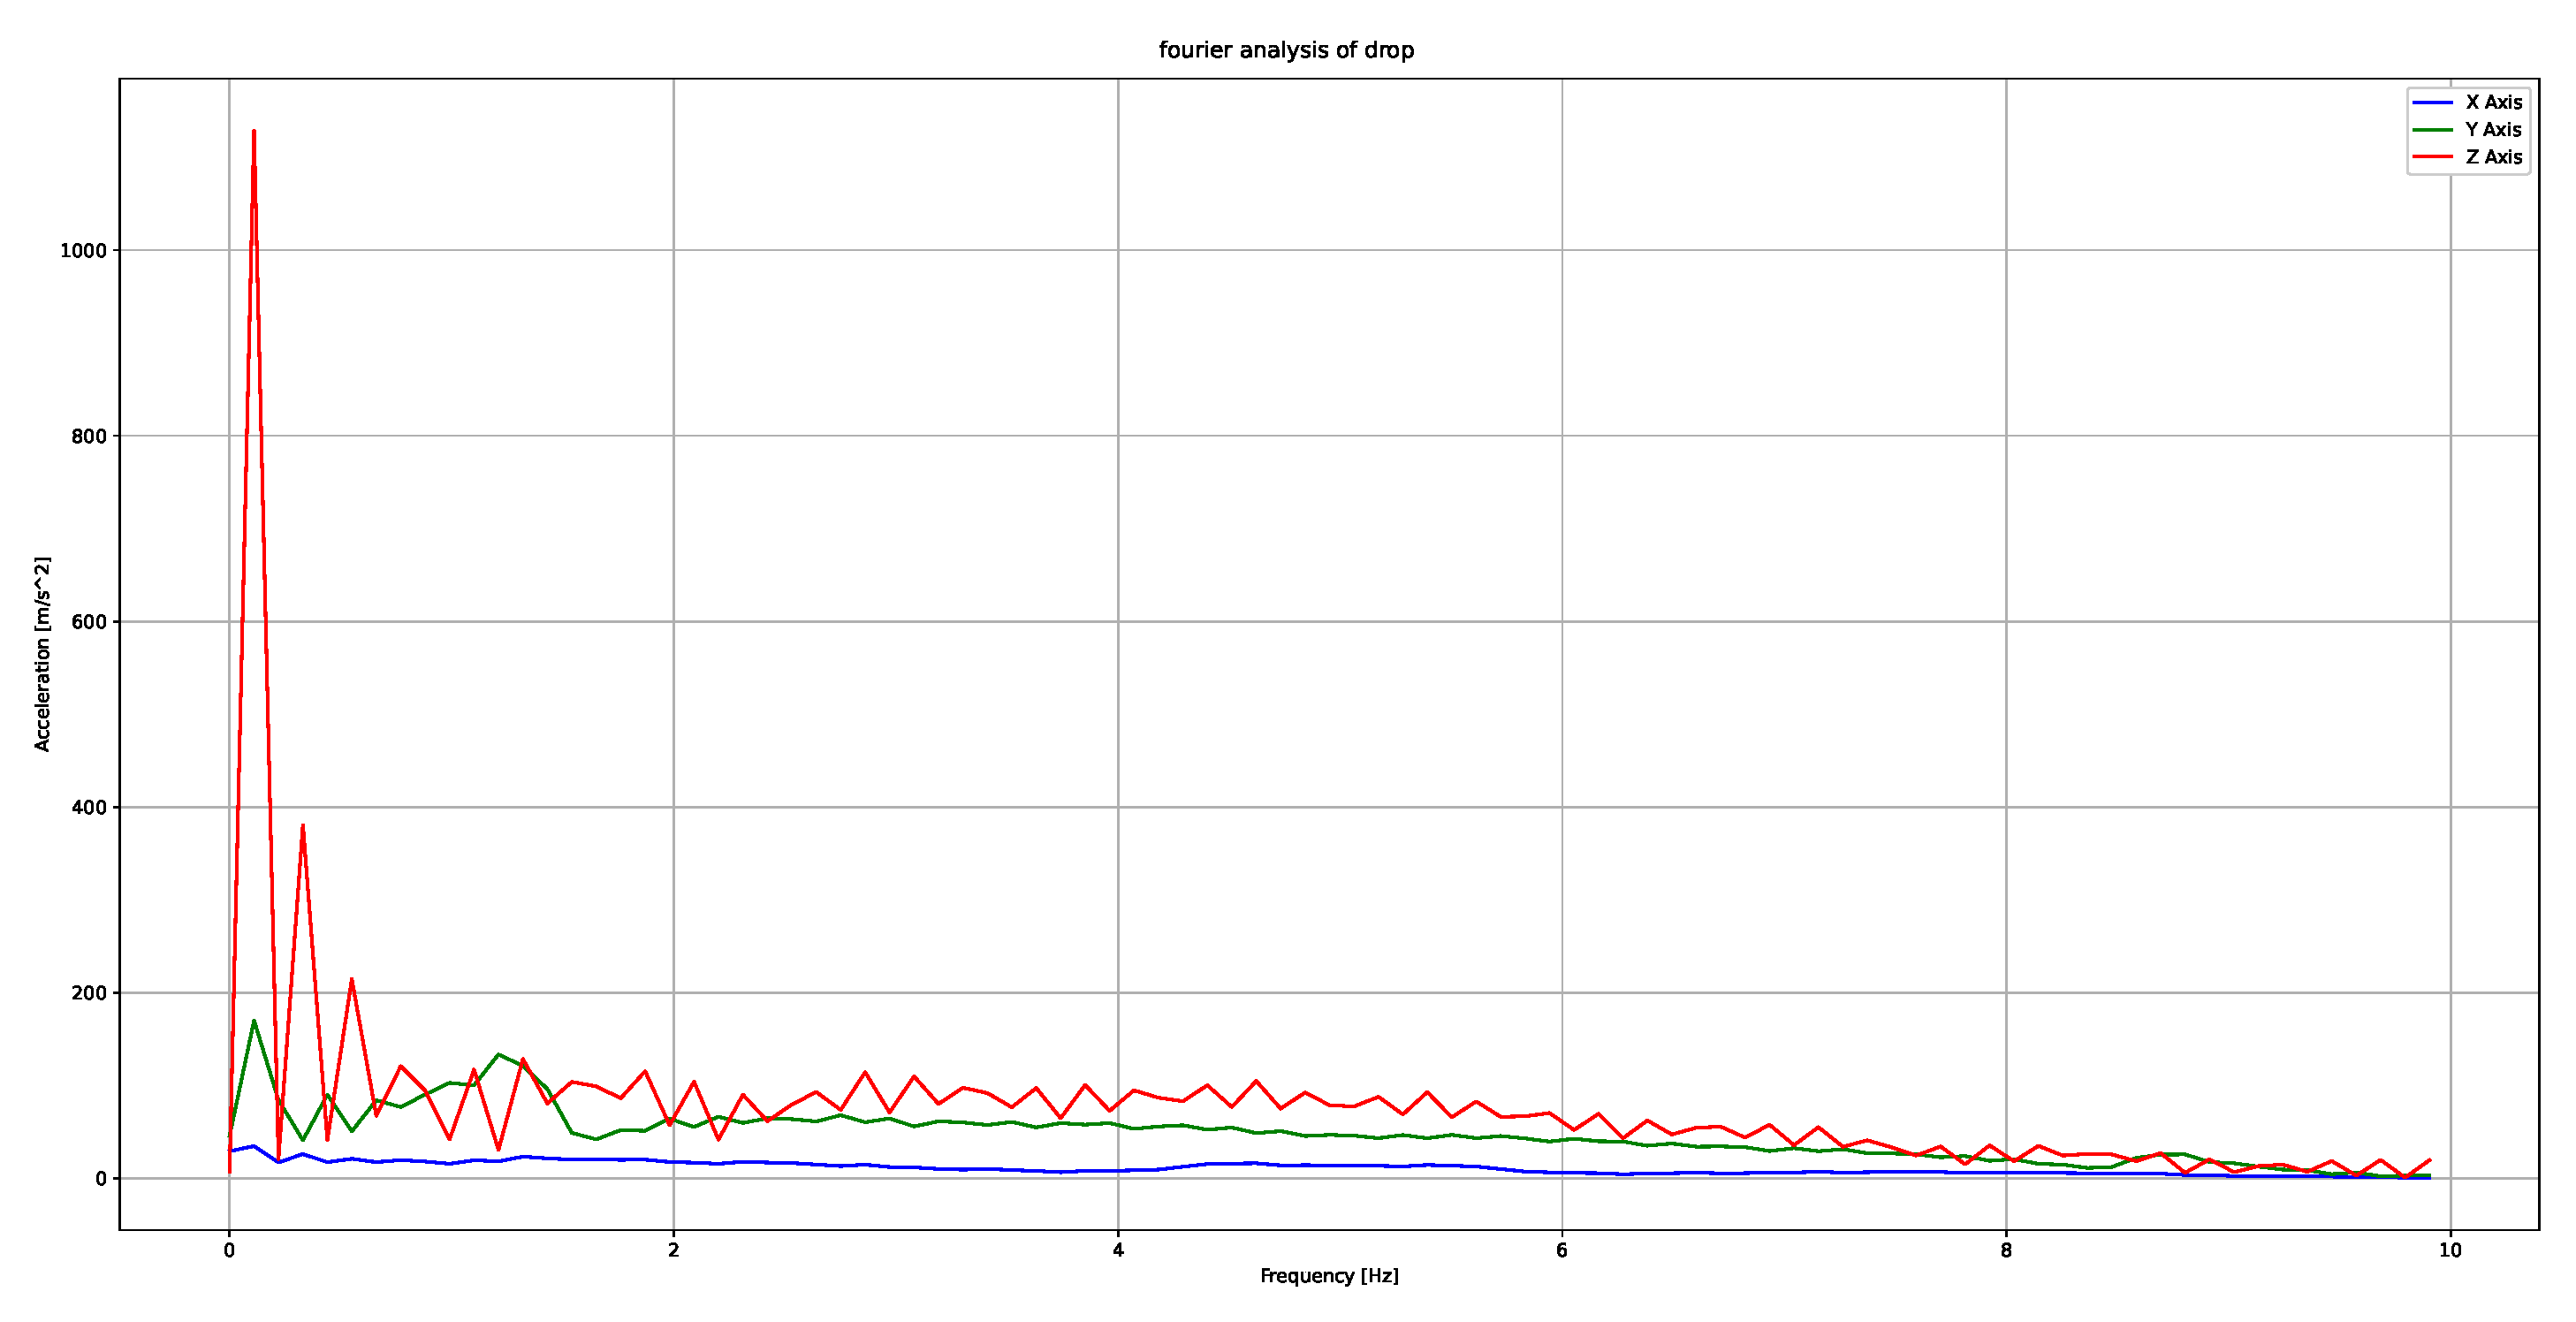
\includegraphics[width=0.8\textwidth]{resources/figures/Fourier_acceleration_drop.eps}
    \caption{Fourier analysis of accelerometer data during the dropping event}
    \label{fig:fourier_accelerometer_dropping}
\end{figure}

\clearpage

\subsubsection{Sawing on the MediColbox}

Figure \ref{fig:accelerometer_sawing} illustrates the
accelerometer data recorded while sawing on the
MediColbox using a metal cutting saw.
The data exhibited periodic variations in acceleration
corresponding to the back-and-forth sawing motion.
The analysis of the data indicated a consistent pattern of
acceleration changes during the sawing event. This suggests that the IMU was able to capture the vibrations and oscillations caused by the sawing action.

\begin{figure}[htbp]
    \centering
    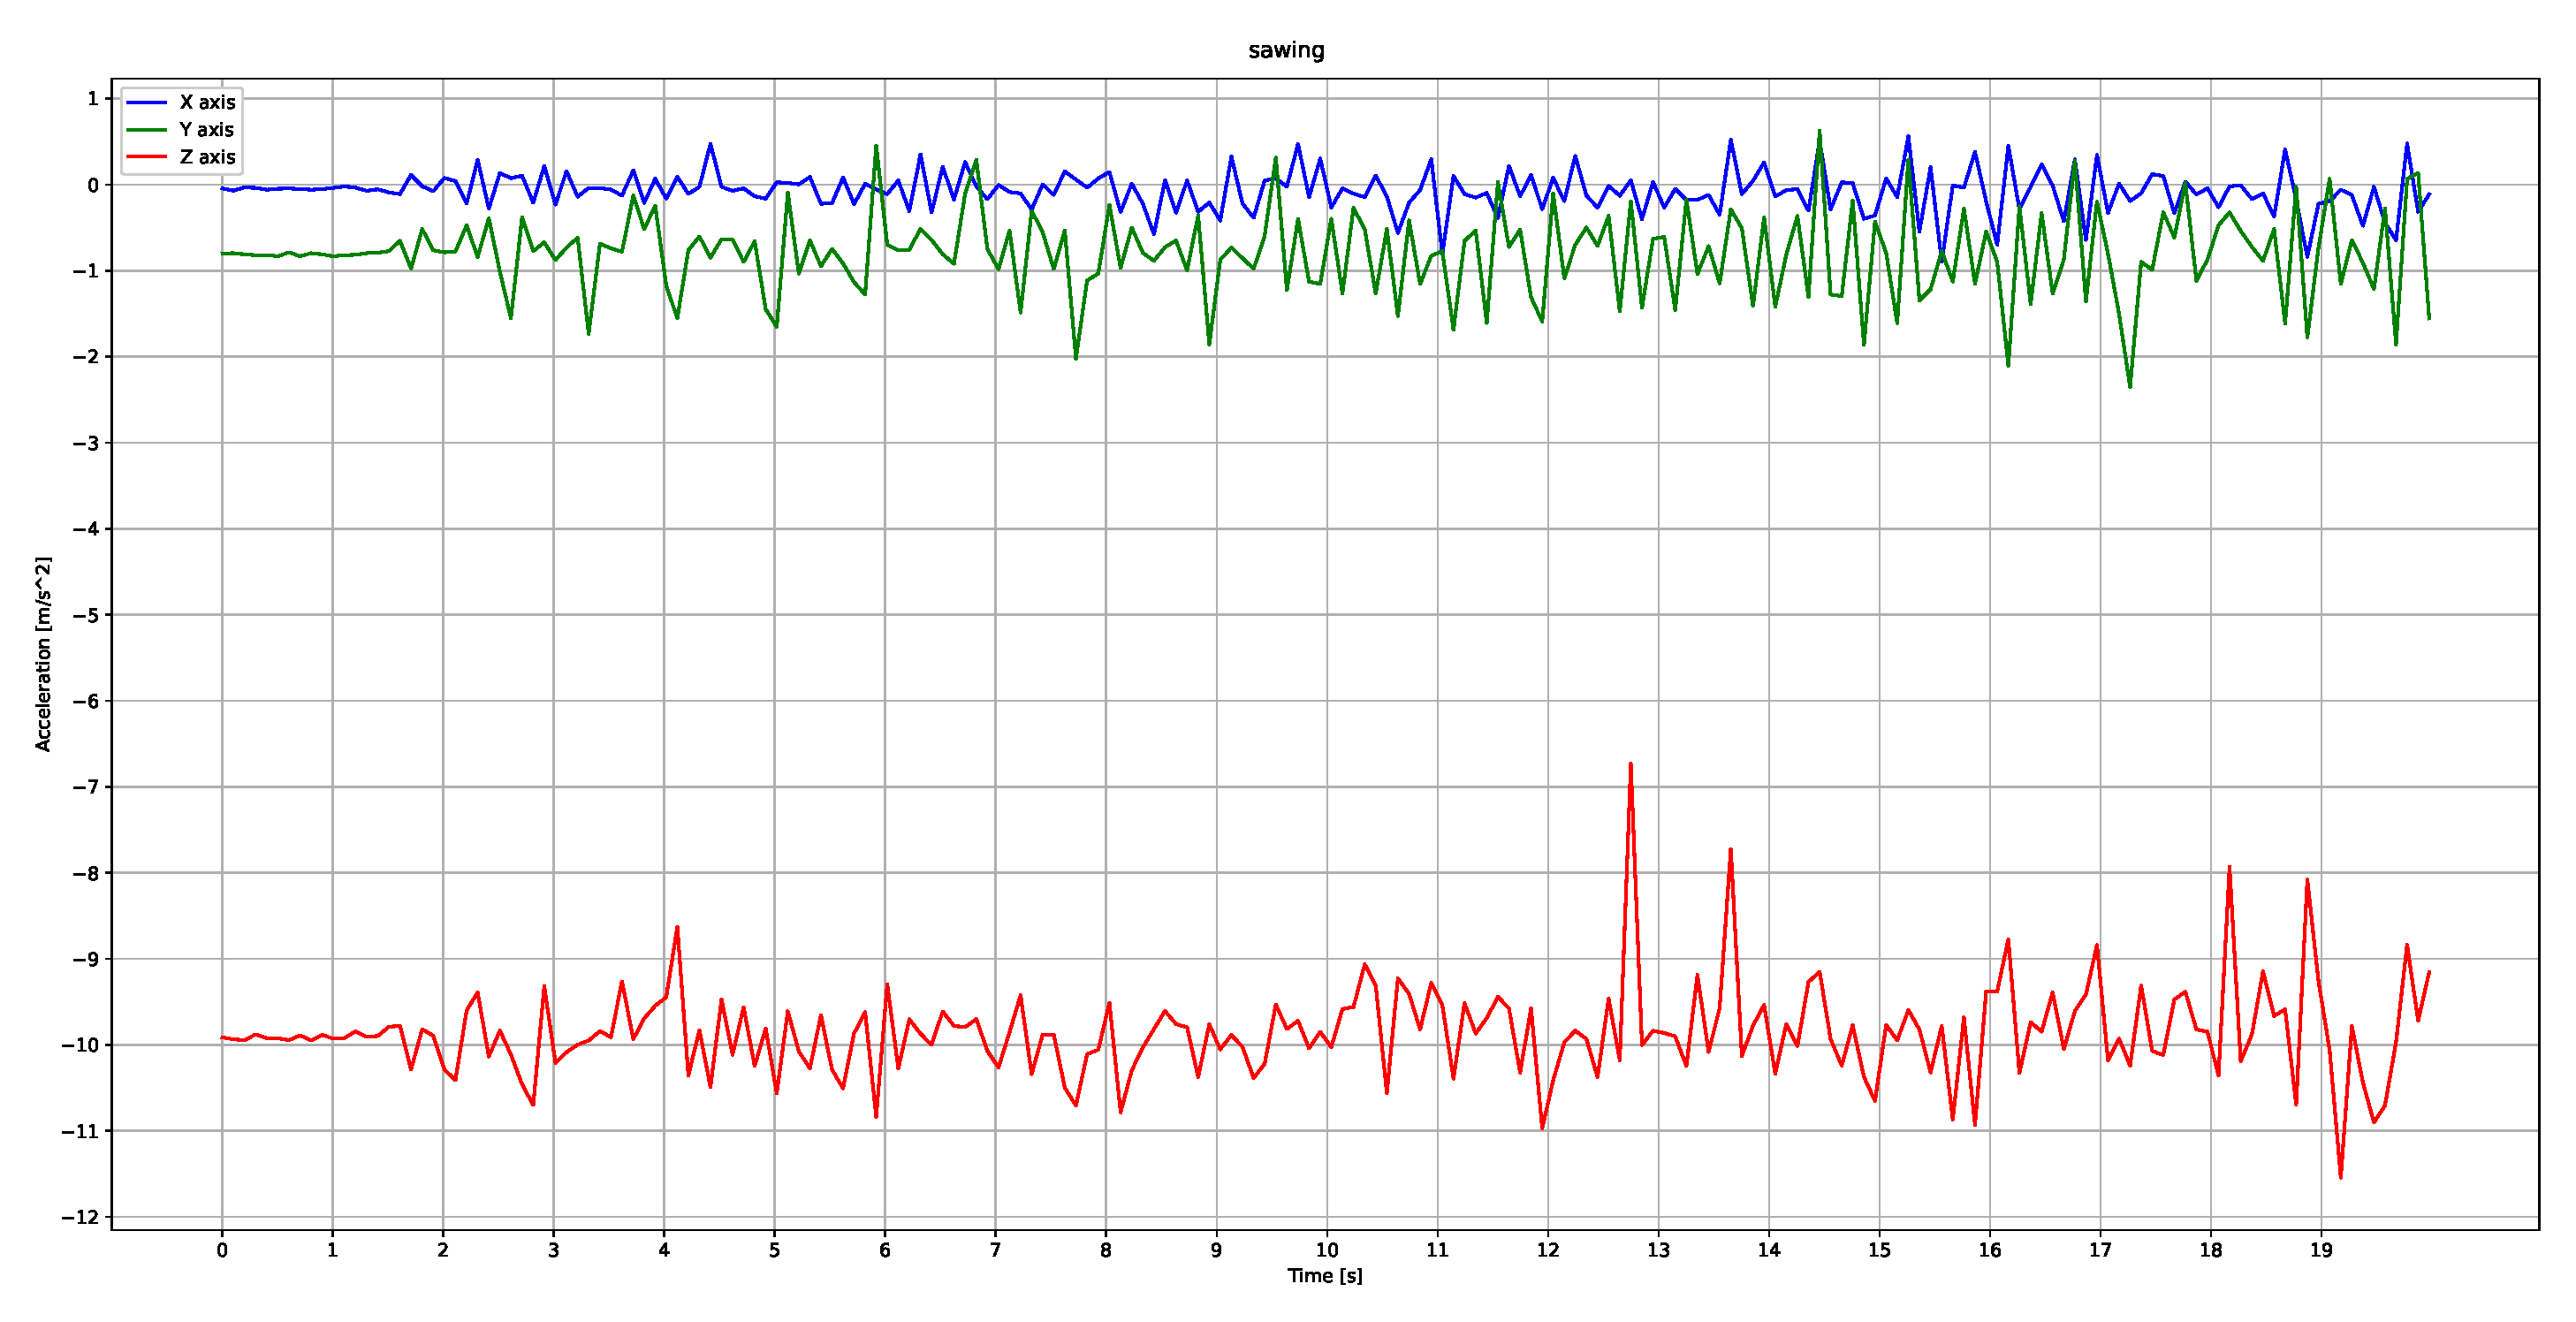
\includegraphics[width=0.8\textwidth]{resources/figures/Acceleration_sawing.eps}
    \caption{Accelerometer data during the sawing event}
    \label{fig:accelerometer_sawing}
\end{figure}

The Fourier analysis of the accelerometer data during the sawing event is shown in Figure \ref{fig:fourier_accelerometer_sawing}. The Fourier analysis allows us to examine the frequency components present in the accelerometer readings and provides insights into the characteristics of the sawing action. By analyzing the frequency distribution and identifying prominent peaks or patterns in the frequency domain, we can gain a deeper understanding of the dynamic response of the MediColbox to the sawing forces.

\begin{figure}[htbp]
    \centering
    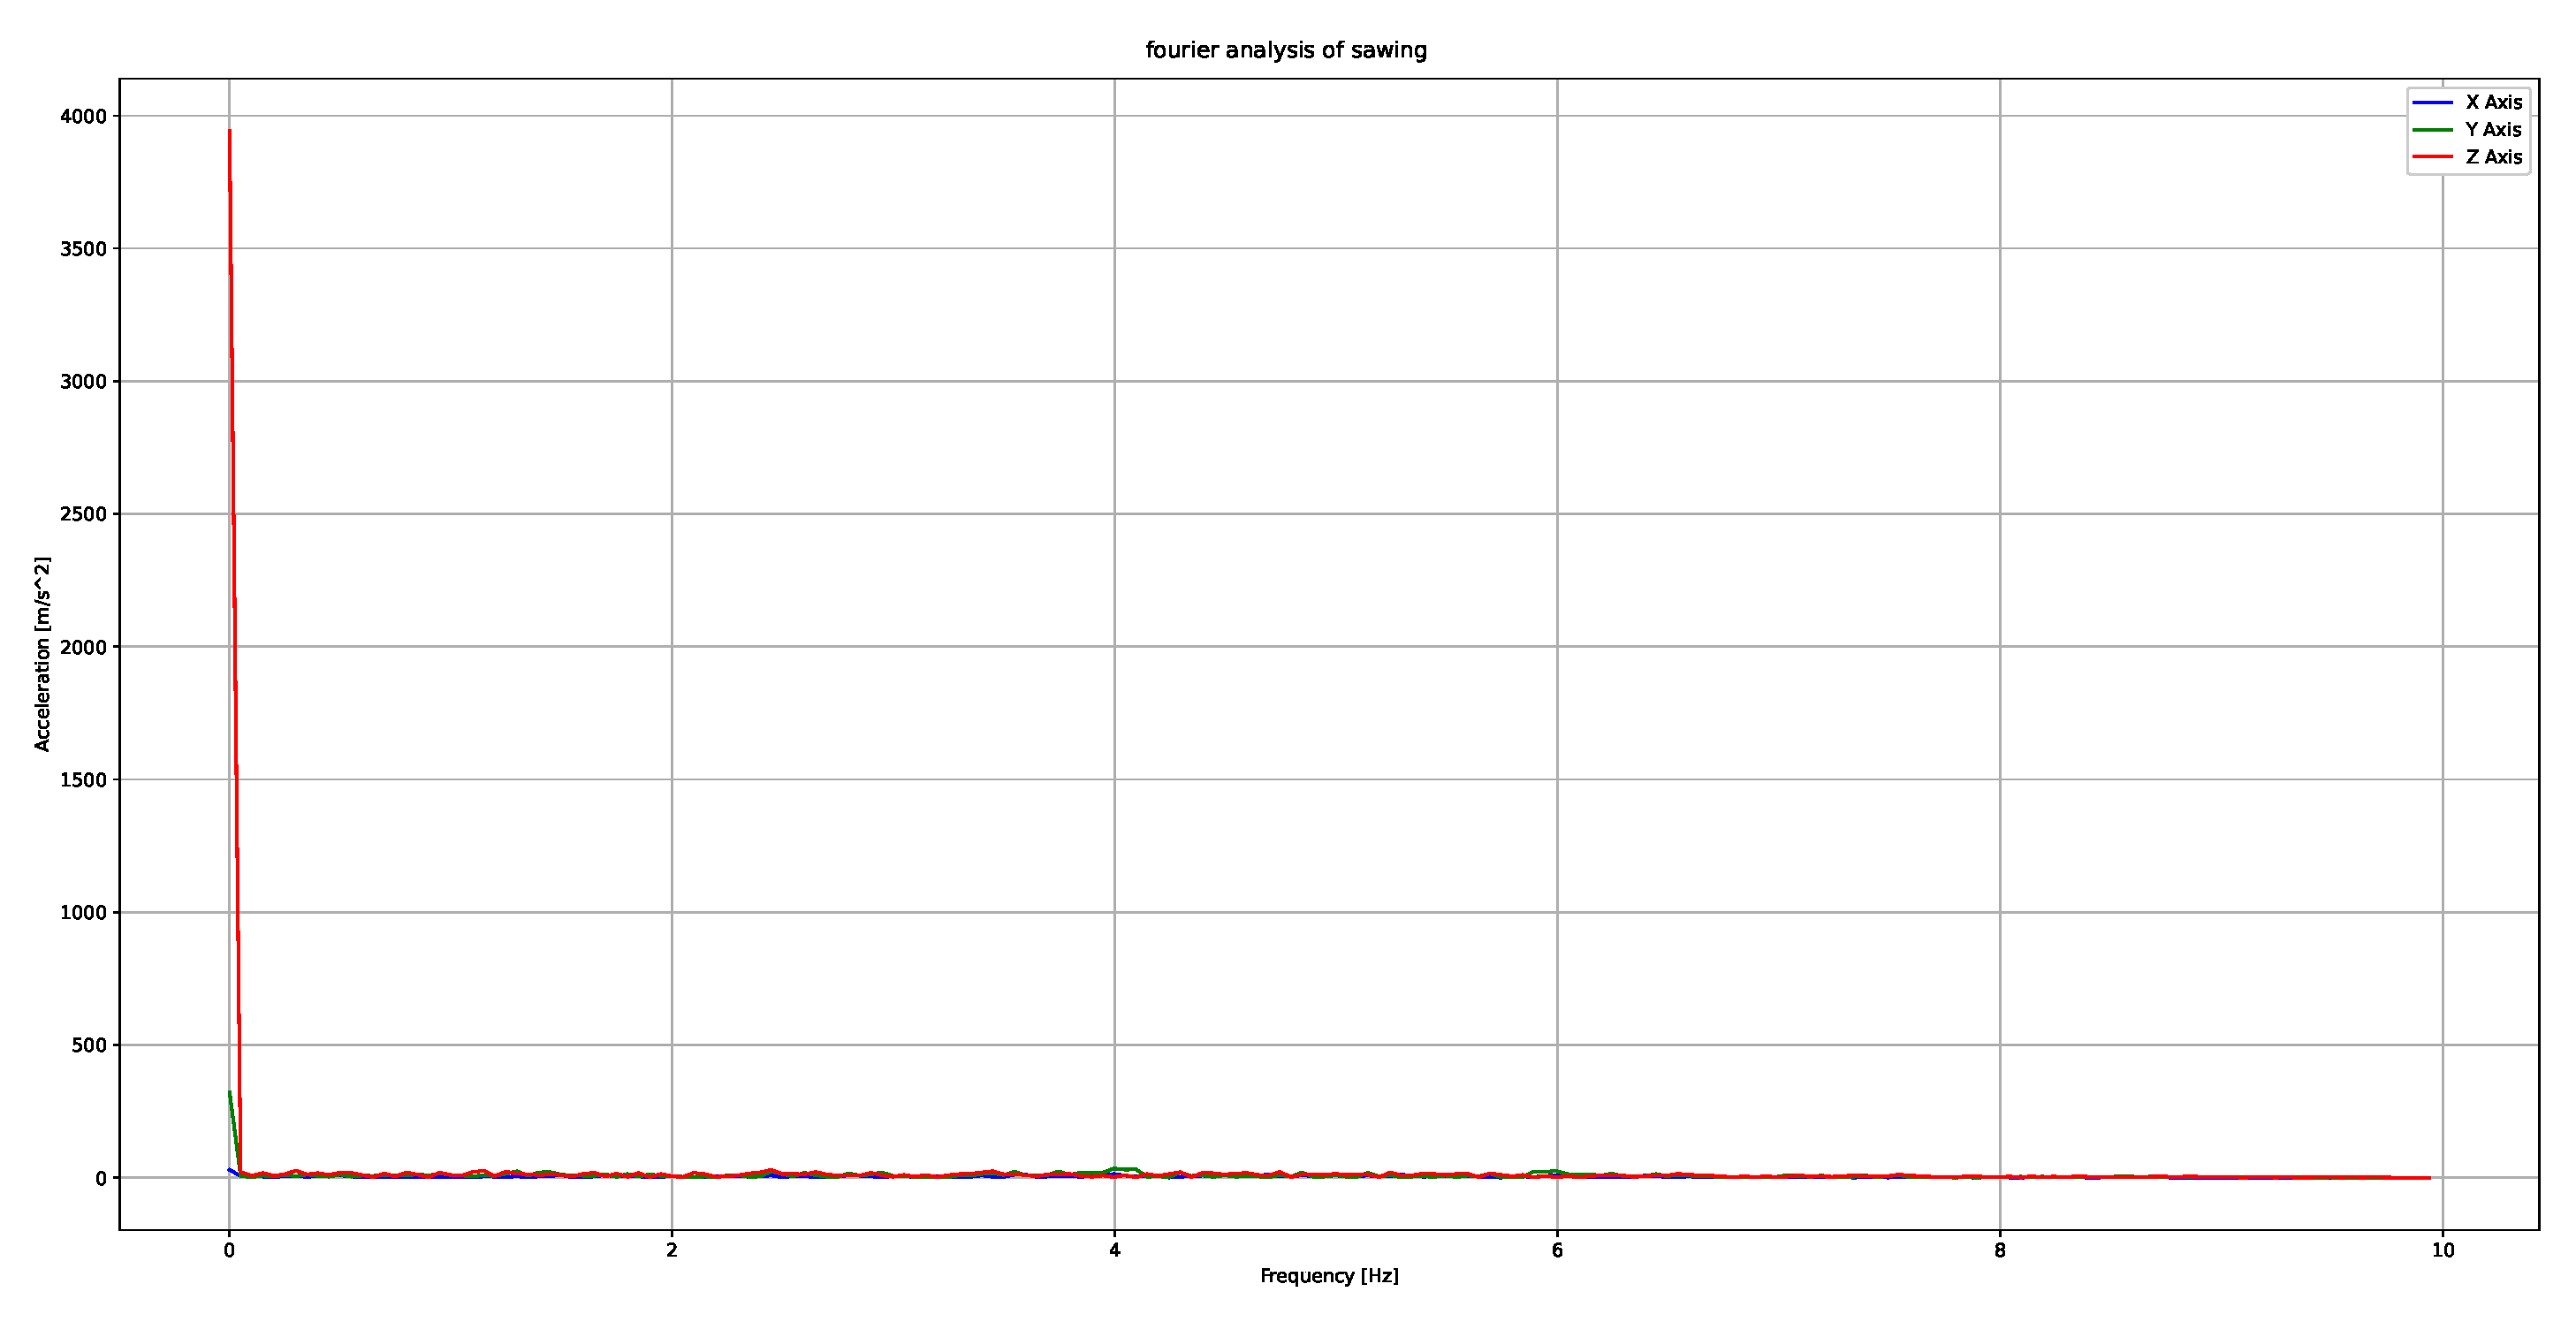
\includegraphics[width=0.8\textwidth]{resources/figures/Fourier_acceleration_sawing.eps}
    \caption{Fourier analysis of accelerometer data during the sawing event}
    \label{fig:fourier_accelerometer_sawing}
\end{figure}

\clearpage

\subsubsection{Shaking the MediColbox}

The accelerometer data obtained while shaking the
MediColbox on a sifter,
simulating cutting it with an angle grinder,
is presented in Figure \ref{fig:accelerometer_shaking}.
The data exhibited irregular and rapid fluctuations in
acceleration due to the shaking motion.
The analysis of the data demonstrated that the IMU was
sensitive enough to detect and record these rapid changes in
acceleration, indicating its potential for
detecting unauthorized access attempts involving
similar movements.

\begin{figure}[htbp]
    \centering
    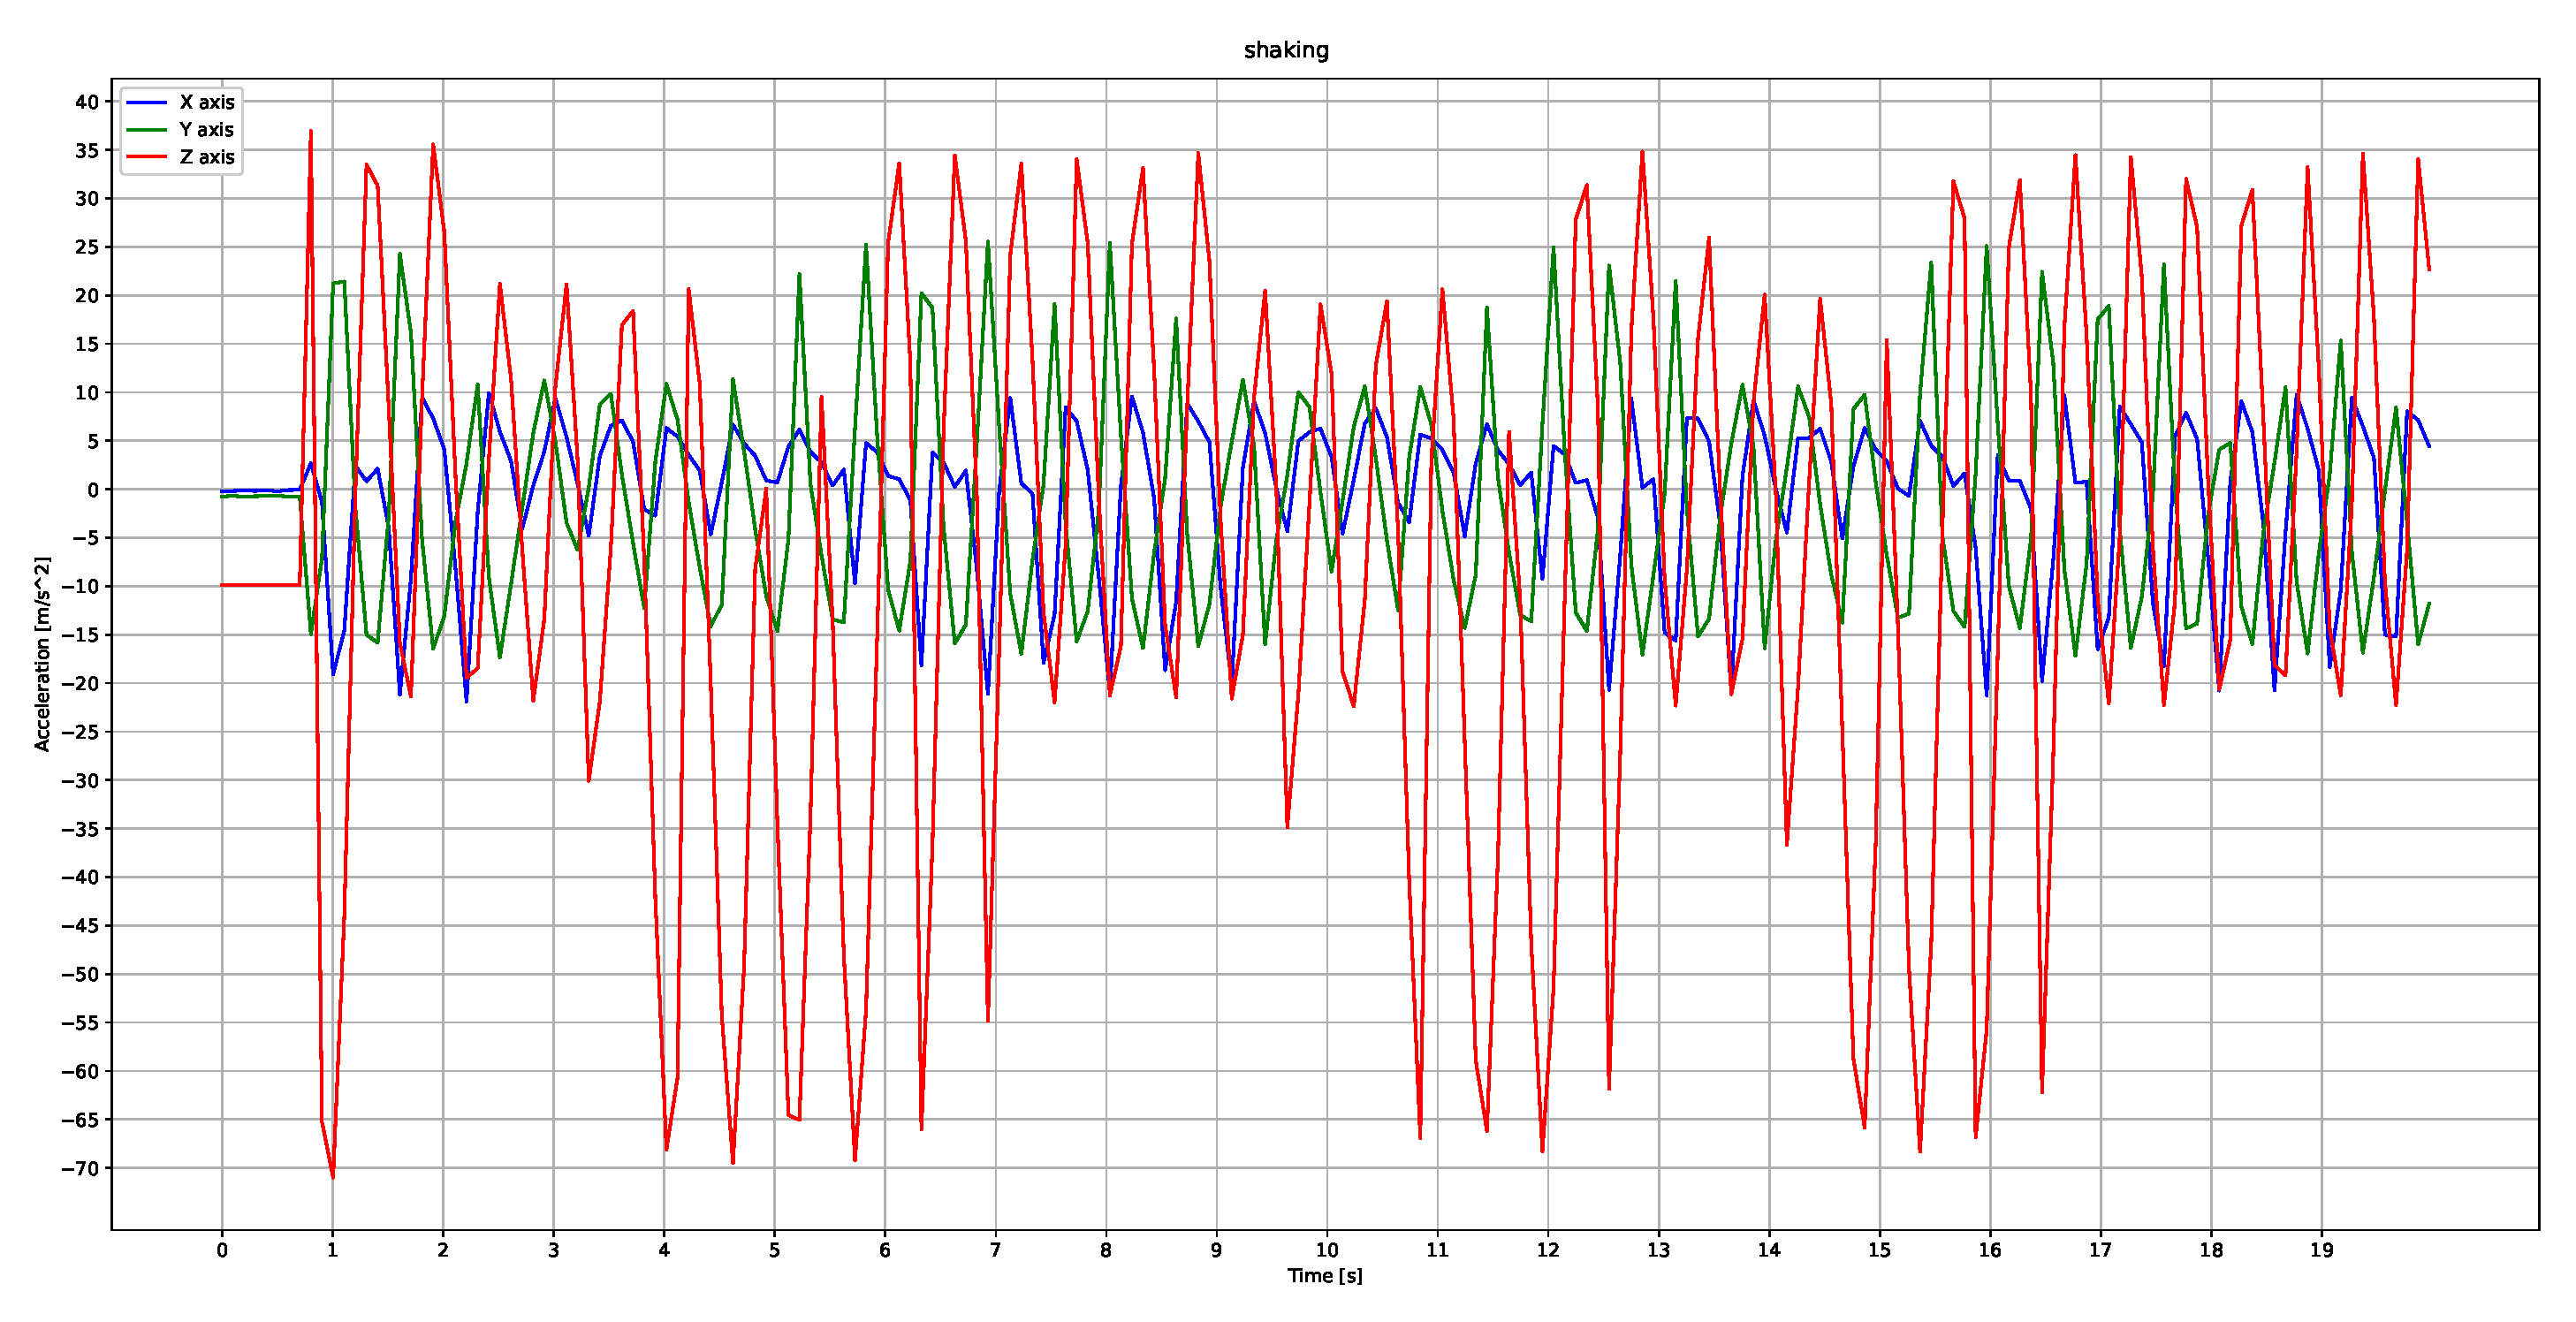
\includegraphics[width=0.8\textwidth]{resources/figures/Acceleration_shaking.eps}
    \caption{Accelerometer data during the shaking event}
    \label{fig:accelerometer_shaking}
\end{figure}

The Fourier analysis of the accelerometer data during the
shaking event is shown in
Figure \ref{fig:fourier_accelerometer_shaking}.
The Fourier analysis allows us to examine the
frequency components present in the accelerometer readings and
provides insights into the characteristics of the shaking motion.
By analyzing the frequency distribution and
identifying prominent peaks or patterns in the frequency domain,
we can gain a deeper understanding of the
dynamic response of the MediColbox to the shaking forces.


\begin{figure}[htbp]
    \centering
    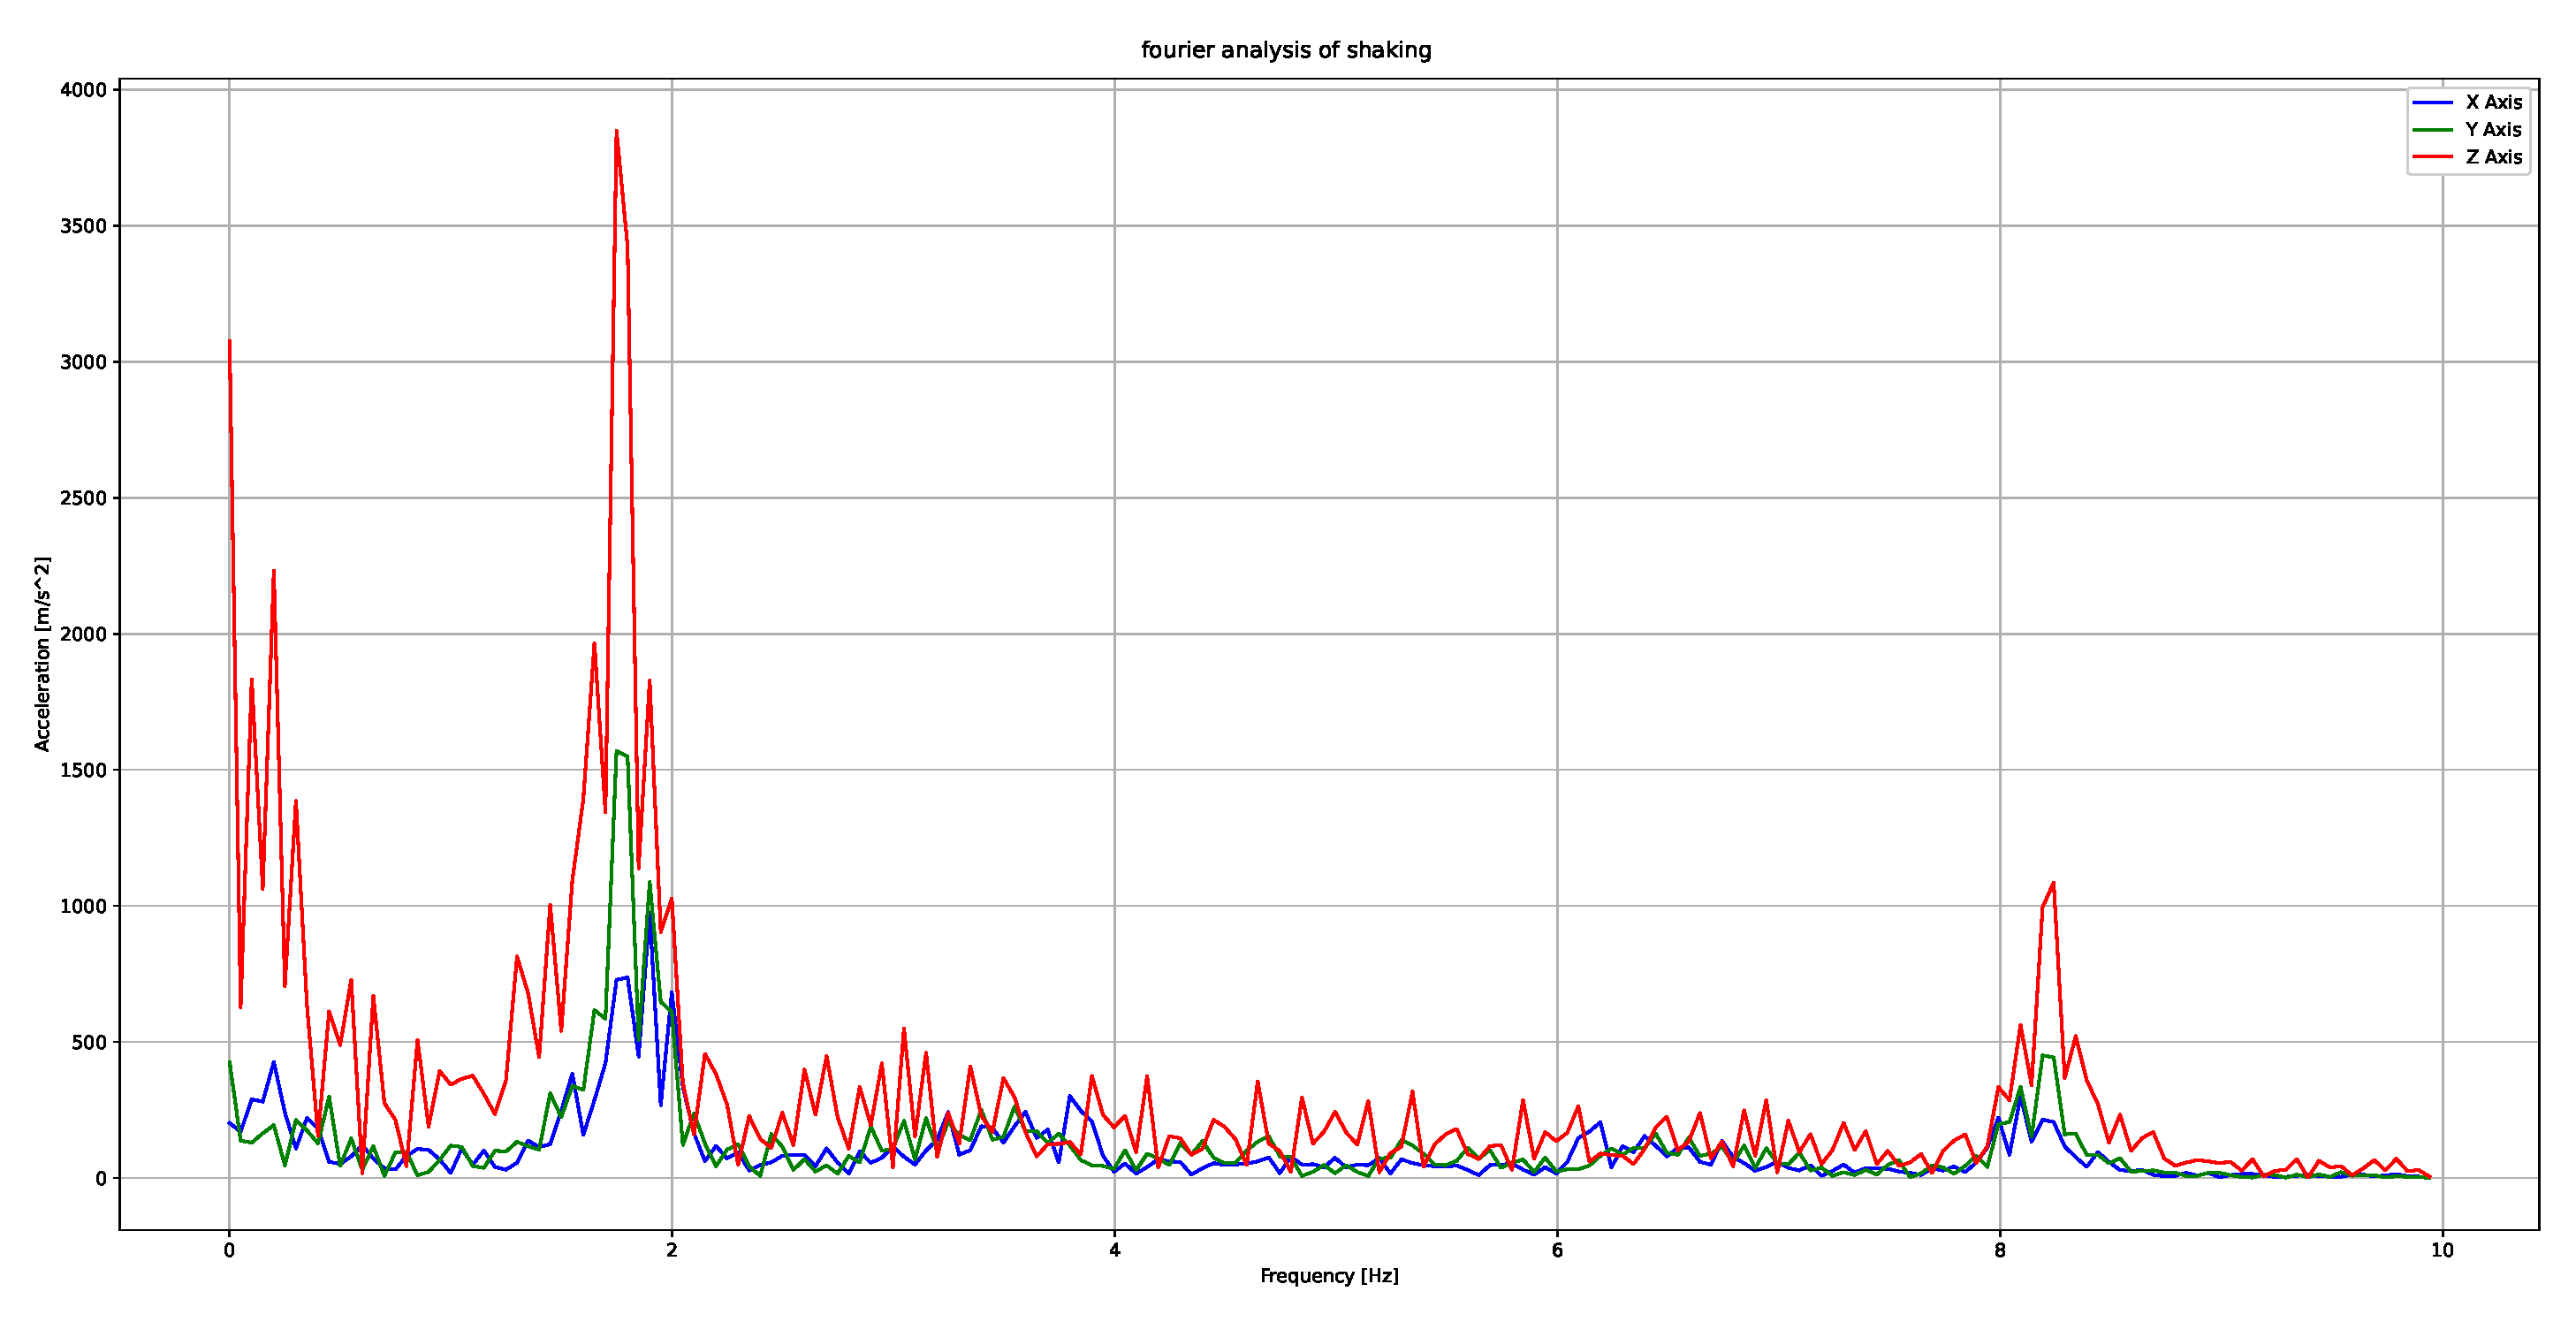
\includegraphics[width=0.8\textwidth]{resources/figures/Fourier_acceleration_shaking.eps}
    \caption{Fourier analysis of accelerometer data during the shaking event}
    \label{fig:fourier_accelerometer_shaking}
\end{figure}

\subsection{Discussion of Findings}

The analysis of the accelerometer data during the
simulated intrusion attempts provides valuable insights into the
IMU's ability to detect and capture unauthorized access events.
The results demonstrate that the
accelerometer readings accurately captured the
accelerative patterns associated with striking,
dropping, sawing, and shaking the MediColbox.

The findings suggest that the IMU is a reliable and
effective sensor for detecting physical movements and vibrations,
which are indicative of intrusion attempts.
The accelerometer data recorded during the
simulated scenarios showcased the IMU's sensitivity to
changes in acceleration,
enabling it to capture both high-impact events and
subtle vibrations.

However, it is important to note that the analysis
focused solely on the accelerometer data,
and other data collected by the IMU,
such as gyroscope or magnetometer readings,
were not considered in this study.
Further research could explore the
integration of multiple sensor data to enhance the
accuracy and robustness of intrusion detection.

Overall, the results indicate the potential of the IMU as
a standalone solution for intrusion detection on the
MediColbox. The findings support the feasibility of
utilizing the IMU to enhance the security and protection of the
MediColbox by effectively detecting and alerting on
unauthorized access attempts.

\end{document}